\documentclass[tikz,border=10pt]{standalone}
\usepackage{amsmath}

\begin{document}
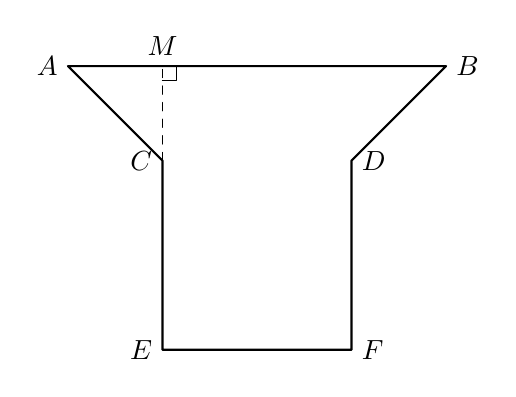
\begin{tikzpicture}[scale=1.2, thick, line join=round, line cap=round]
    
    % --- 1. 坐标定义 ---
    \coordinate (A) at (-2, 3);
    \coordinate (B) at (2, 3);
    \coordinate (C) at (-1, 2);
    \coordinate (D) at (1, 2);
    \coordinate (E) at (-1, 0);
    \coordinate (F) at (1, 0);
    \coordinate (M) at (-1, 3); % 垂足 M

    % --- 2. 绘制轴截面轮廓 ---
    \draw (A) -- (B) -- (D) -- (F) -- (E) -- (C) -- cycle;

    % --- 3. 绘制辅助线和直角符号 ---
    \draw[dashed, thin] (C) -- (M);
    % 绘制直角标志
    \draw[thin] (-1, 2.85) -- (-0.85, 2.85) -- (-0.85, 3);

    % --- 4. 节点字母标定 ---
    \node[left] at (A) {$A$};
    \node[right] at (B) {$B$};
    \node[left] at (C) {$C$};
    \node[right] at (D) {$D$};
    \node[left] at (E) {$E$};
    \node[right] at (F) {$F$};
    \node[above] at (M) {$M$};

\end{tikzpicture}
\end{document}